Program dites menggunakan dua masukan. Yang pertama, program dites menggunakan masukan yang tidak \textit{valid}, yaitu AAA. Hasilnya adalah :
\begin{figure}[h!]
  \centering
  \caption{Tes pertama, masukan tidak \textit{valid}}.
  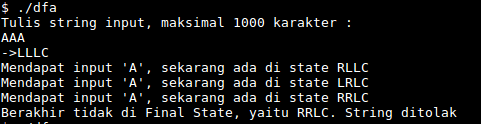
\includegraphics[width=350pt]{AAA.png}
\end{figure}

Lalu, program dites menggunakan masukan yang \textit{valid}, yaitu AAB. Hasilnya adalah :
\begin{figure}[h!]
  \centering
  \caption{Tes kedua, masukan \textit{valid}}.
  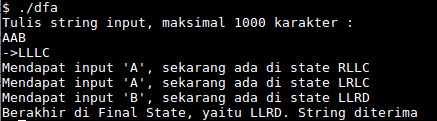
\includegraphics[width=350pt]{AAB.png}
\end{figure}

Dari kedua tes tersebut, didapat bahwa program melakukan simulasi \textit{state-state} yang dilalui dengan benar. Selain itu, program juga memberikan kesimpulan tentang diterima atau tidaknya sebuah masukan dengan benar.
